\documentclass[12pt,a4paper,ngerman]{article}
\usepackage{stylesheet}
\begin{document}
\TUHeader                          %  Bitte Ausfüllen!!!
%----------------------------
{Übung F: Übertragungsverhalten nachrichtentechnischer Systeme}                       %  Übungstitel
%----------------------------
{25.11.2014}                        %  Übungsdatum
%----------------------------
{05}                            %  Gruppen-Nr.
%----------------------------
{Thomas Neff}                   % Name des Protokollführers
%----------------------------
{
1.~Daniel Freßl, 1230028\\
2.~Thomas Neff, 1230319\\                    %  Übungsteilnehmer
3.~Thomas Pichler, 1230320 \\                   %  ...bei <4 Teilnehmer auskommentieren
4.~Martin Winter, 1130688\\
5.~Bernadette Schreyer, 1073076\\
}
%----------------------------
{Ao.Univ.-Prof. Dipl.-Ing. Dr. techn. Erich Leitgeb}
{Max Henkel}                          %  Betreuer
%----------------------------
{Graz}                              %  Ort der Protokollerstellung
{\today}                            %  Datum Protokollerstellung




\pagebreak
  
\tableofcontents
  
\pagebreak

%-------------------------------------------------------------------------------
%
% Beginn des Protokolls
%
%-------------------------------------------------------------------------------

\section*{Task-Ausführung}


\begin{framed}
Beschäftigen Sie sich mit der Ausführung von Tasks durch ein Echtzeitbetriebssystem. Nennen sie die Unterschiede zwischen synchroner und asynchroner Taskausführung. Überlegen Sie sich zu beiden Arten jeweils mindestens 2 Beispiele anhand derer sie die jeweiligen Funktionsweise genau erklären. Gehen sie in den Beispielen ebenfalls auf Minor und Major Frames ein, sowie auf die Zeitbedingungen. 
\end{framed}
Nicht bearbeitet. 
\pagebreak
\section*{Schedulingverfahren}


\begin{framed}
Klassifizieren Sie die Schdeduling-Algorithmen \textbf{EDF}, \textbf{EDD}(Earliest Deadline Due), \textbf{RMS}, \textbf{DMS} (Deadline Monotonic Scheduling), \textbf{FCFS} und \textbf{RR} (RoundRobin) bezüglich folgender Kriterien:
\begin{itemize}
\item hart-echtzeitfähig vs zeit-unkritisch
\item periodisch vs aperiodisch vs hybrid
\item preemptive vs non-preemptive
\item statisch vs dynamisch
\item on-line vs off-line
\end{itemize}
Welche Kombination von Scheduling-Algorithmen würden Sie verwenden, um hart-echtzeitfähige periodische Tasks zusammen mit sporadischen (aperiodischen) auszuführenden, aber zeitunkritischen Tasks in sogenannten "offenen Systemen" zu planen?
\end{framed}



\textbf{EDF} (Earliest Deadline first)\\
Ist ein \textbf{dynamisches} Schedulingverfahren, bei jedem Schedulingevent wird in der List der Task mit nächsten Deadline gesucht und dieser dann ausgeführt. Es ist eher \textbf{hart-echtzeitfähig}, aber es ist nicht leicht nachvollziehbar ist, ob Deadlines eingehalten werden oder nicht. Es handelt sich um ein \textbf{preemptives} Verfahren, welches mit periodischen, als auch aperiodischen Task gut klarkommt, also \textbf{hybrid}. 
\\
\textbf{EDD} (Earliest Deadline due) 
Ist ein \textbf{statisches }Schedulingverfahren, hierbei wird ähnlich wie bei EDF gearbeitet, nur das keine dynamischen Ändernungen möglich sind. Es ist also ebenso ebenso \textbf{hart-echtzeitfähig}, \textbf{preemptive} und \textbf{hybrid}. \\
\textbf{RMS} (Rate-Monotonic Scheduling) \\
Hier werden die die Prioritäten zur Design-Zeit festgelegt nach zunehmenden Taskperioden, je kürzer die Periodendauer eines Prozesses, desto höher ist seine Priorität, es ist also \textbf{statisch}. 
Hierbei wird immer der Prozess mit der höchsten Priorität gescheduled, es ist also \textbf{hart-echtzeitfähig}, \textbf{preemptive} und kann sowohl mit periodischen, also auch aperiodischen Taks umgehen, ist also \textbf{hybrid}.  \\
\textbf{DMS} (Deadline Monotonic Scheduling) \\
Dies ist ein 	Verfahren, das \textbf{harte echtzeitfähig} ist, es dient zur Verwaltung von Prozessen mit fester Priorität.
Prozesse können hierbei zu jeder Zeit unterbrochen werden, es ist also \textbf{preemptive}. Es wird, wie bei RMS stets der Prozess der höchsten Priorität ausgeführt. Aperiodische Prozesse können auch eingebaut werden, indem man diese als fiktive periodische Prozesse integriert, das Verfahren ist also \textbf{hybrid}.  Es vergibt dabei fixe Prioritäten, ist also \textbf{statisch}.\\
\textbf{FCFS} (FIFO) \\
Bei FIFO werden Prozesse einfach so angeordnet, wie sie in der Ready-Schlange ankommen, es ist ein Verfahren mit \textbf{statischen bzw. keinen} Prioritäten, wer zuerst bereit ist, wird gescheduled, es ist auch \textbf{non-preemptive}, Task laufen so lange, bis sie fertig sind, kann somit zu Starvation führen. Dadurch ist auch das ganze Verfahren \textbf{dynamisch} und nur \textbf{zeitunkritisch}, da auch die Prozesse in jeder Reihenfolge dran kommen können, ist es \textbf{aperiodisch}.  \\
\textbf{RR} (RoundRobin)\\
Jeder Prozess bekommt einen fixen Zeitslot und so wird durch rotiert zwischen den Prozessen, es handelt sich somit um ein \textbf{statisches Verfahren}. 
Ist ein  Schedulingverfahren mit \textbf{statischen bzw. keinen} Prioritäten, Tasks werden immer im Kreislauf gescheduled, es handelt sich also um ein \textbf{periodisches} Verfahren, welches \textbf{preemptive} ist, Task werden nach einer gewissen Zeit unterbrochen und der nächste Task kommt dran. Dadurch lässt sich natürlich keine harte Echtzeitfähigkeit garantieren, es handelt sich also um ein \textbf{zeitunkritisches} Verfahren. Hierbei kann es aber zu keiner Starvation kommen, da keine Priorität vergeben wird. \\

\vspace{0.5cm}
Für dieses offene System würde sich entweder RMS oder DMS anbieten, da beide sehr gut mit hart echtzeitfähigen, periodischen Prozessen umgehen können, aber auch aperiodische gut integrieren können. 


\pagebreak

\section*{Anwendungsbeispiel Scheduling-Verfahren}


\begin{framed}
Bearbeiten Sie für die unten angegebenen Beispiele zur Prioritätsvergabe folgene Aufgaben mittels Rate-Monotonic Scheduling (RMS)
\begin{itemize}
\item Zeigen Sie, unter Zuhilfenahme des in der VO gezeigten Satzes, ob ein RM-Schedule sicher existiert oder nur möglicherweise.
\item Zeigen Sie wie ein mögliches RM-Scheduling aussehen könnte, falls kein RM Schedule möglich ist, zeigen sie, wo es zu Problemen kommt. 
\item Versuchen Sie Problemfälle unter Zuhilfenahme eines anderen, in der VO gezeigten, dynamischen Schedulingverfahrens zu lösen. 
\end{itemize}


\end{framed}
\begin{table}[h!]
  \begin{center}
    \begin{tabular}{c c c c c c c}
    \toprule
    Task &Bsp & 1 & Bsp & 2 & Bsp & 3  \\ \midrule
     1 & C & T & C & T & C & T  \\
     A & 1 & 5 & 1 & 4 & 1 & 4 \\
     B & 1 & 7 & 1 & 7 & 1 & 5 \\
     C & 2 & 10 & 2 & 8 & 2 & 8 \\
     D & 2 & 15 & 2 & 13 & 2 & 10 \\
     E & 1 & 16 & 1 & 14 & 1 & 12\\    
      \bottomrule
    \end{tabular}
  \end{center}
\end{table}
Nach dem Satz in der VO gibt es dann ein garantiertes Scheduling, wenn folgendes gilt
\begin{equation}
\sum_{i=1}^{n}{\frac{C_i}{T_i}} \leq n \cdot \left(\sqrt[n]{2}-1\right)
\end{equation}
Damit ergibt sich für die 3 Beispiele
\begin{align*}
U_1 &= \frac{1}{5} + \frac{1}{7} + \frac{ 2}{10} + \frac{2}{15} + \frac{1}{16} = 0.73869 \leq 0.74349 \\
U_2 &= \frac{1}{4} + \frac{1}{7} + \frac{2}{8} + \frac{2}{13} + \frac{1}{14} = 0.86813 \geq 0.74349\\
U_3 &= \frac{1}{4} + \frac{1}{5} + \frac{2}{8} + \frac{2}{10} + \frac{1}{12} = 0.98333333 \geq 0.74349
\end{align*}

\pagebreak
\begin{figure}[h!]
\centering
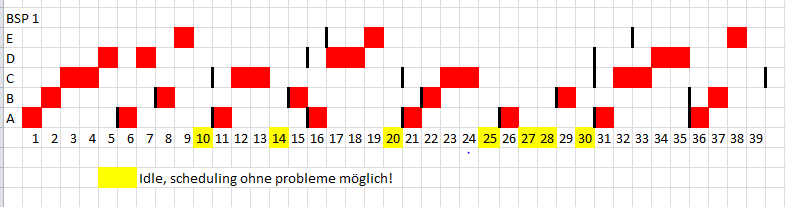
\includegraphics[width=\columnwidth]{figures/bsp1.jpg} 
\end{figure}
\begin{figure}[h!]
\centering
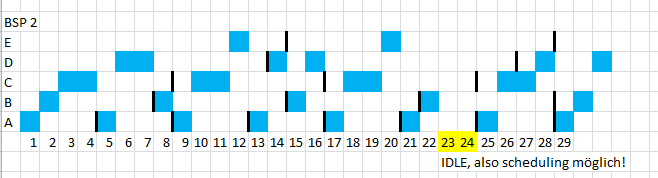
\includegraphics[width=\columnwidth]{figures/bsp2.jpg} 
\end{figure}
\begin{figure}[h!]
\centering
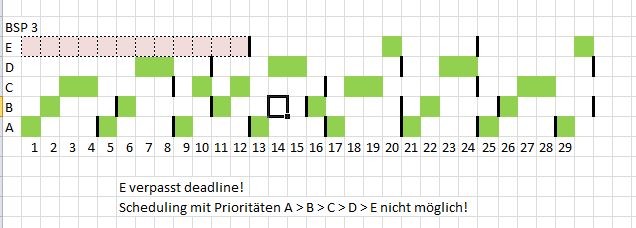
\includegraphics[width=\columnwidth]{figures/bsp3.jpg} 
\end{figure}
Die Probleme beim letzen Beispiel würden sich lösen lassen, wenn man EDF (Earliest Deadline First) verwenden würde. 
\pagebreak

\section*{Anwendung von Scheduling}


\begin{framed}
Gegeben seien folgende Tasks, deren Periode und Ausführungszeit
\begin{itemize}
\item Task 1 = (3;6)
\item Task 2 = (2;9)
\item Task 3 = (k, 12)
\end{itemize}
Wählen sie k so, dass die Tasks mittels EDF und RMS
\begin{itemize}
\item auf keinen Fall schedulbar sind
\item eventuell schedulbar sind
\item auf jeden Fall schedulbar sind
\end{itemize}
Analysieren Sie alle 3 Fälle für beide Algorithmen und begründen sie jeweils die Wahl von k. 
\end{framed}

\begin{align*}
U_1 = \frac{C_1}{T_1} = \frac{3}{6} = \frac{1}{2}; \quad U_2 = \frac{C_2}{T_2} = \frac{2}{9}; \quad
U_3 = \frac{C_3}{T_3} = \frac{k}{12} \\
U = \sum_{j=1}^{n} \frac{C_j}{T_j} = \frac{1}{2} + \frac{2}{9} + \frac{k}{12} = \frac{3k+26}{36}
\end{align*}
die Prozessorauslastung U muss $\leq 1$ sein, damit sich das Verfahren ausgeht, somit gilt: \\
\textbf{EDF (Earliest Deadline First)}: \\
\begin{itemize}
\item auf keinen Fall schedulbar $\Rightarrow \quad k > 3.334$
\item eventuell schedulbar $\Rightarrow \quad$ hier nicht vorhanden
\item auf jeden Fall schedulbar $\Rightarrow \quad k \leq 3.334$
\end{itemize}
\textbf{RMS (Rate-Monotonic Scheduling)}: \\
\begin{align*}
U_g &= n(2^{\frac{1}{n}}-1) = 3 (2^{\frac{1}{3}}-1) = 0.78 \\
U &= \frac{3k+26}{36} \leq 0.78 \quad \Rightarrow \quad k \leq 0.69
\end{align*}
Wenn $U\leq U_g(n)$ (in diesem Fall n=3), ist, dann existiert immer ein RM-Schedule!
\begin{itemize}
\item auf keinen Fall schedulbar $\Rightarrow \quad k > 3.334$
\item eventuell schedulbar $\Rightarrow \quad 0.69 < k \leq 3.334$
\item auf jeden Fall schedulbar $\Rightarrow \quad k \leq 0.69$
\end{itemize}




   
   
\end{document}